\documentclass[11pt,tikz,border=2mm]{standalone}
\usepackage{csquotes}
\usepackage[backend=biber,style=numeric,sorting=none]{biblatex}

\usepackage{siunitx}
\usepackage{tikz}
\usepackage[siunitx,american]{circuitikz}
\usepackage{pgfplots}
\usepackage{amsmath}
\usepackage{tikz-3dplot}

\usetikzlibrary{decorations.pathmorphing,patterns}
\usetikzlibrary{shapes.geometric, arrows}
\usetikzlibrary{positioning}
\usetikzlibrary{3d}
\usepgfplotslibrary{units}
\usepgfplotslibrary{groupplots}
\pgfplotsset{compat=1.18}

\ctikzset{tripoles/mos style/arrows}

\definecolor{IBM1}{HTML}{648fff}%blå
\definecolor{IBM2}{HTML}{785ef0}%blå
\definecolor{IBM3}{HTML}{dc267f}%rød
\definecolor{IBM4}{HTML}{fe6100}%orange
\definecolor{IBM5}{HTML}{ffb000}%gul
\definecolor{IBM6}{HTML}{d55e00}%orange-brun
\definecolor{IBM7}{HTML}{cc79a7}%lilla
\definecolor{IBM8}{HTML}{0072b2}%blågrøn
\definecolor{IBM9}{HTML}{f0e442}%gul
\definecolor{IBM10}{HTML}{009e73}%grøn

\tikzstyle{solid}=                   [dash pattern=]
\tikzstyle{dotted}=                  [dash pattern=on \pgflinewidth off 2pt]
\tikzstyle{densely dotted}=          [dash pattern=on \pgflinewidth off 1pt]
\tikzstyle{loosely dotted}=          [dash pattern=on \pgflinewidth off 4pt]
\tikzstyle{dashed}=                  [dash pattern=on 3pt off 3pt]
\tikzstyle{densely dashed}=          [dash pattern=on 3pt off 2pt]
\tikzstyle{loosely dashed}=          [dash pattern=on 3pt off 6pt]
\tikzstyle{dashdotted}=              [dash pattern=on 3pt off 2pt on \the\pgflinewidth off 2pt]
\tikzstyle{densely dashdotted}=      [dash pattern=on 3pt off 1pt on \the\pgflinewidth off 1pt]
\tikzstyle{loosely dashdotted}=      [dash pattern=on 3pt off 4pt on \the\pgflinewidth off 4pt]

\providecommand{\PlotFont}{\normalsize}
\providecommand{\PlotWidth}{12cm}
\providecommand{\PlotHeight}{7cm}
\pgfplotsset{every axis/.append style={font=\PlotFont, width=\PlotWidth, height=\PlotHeight}}

\DeclareSIUnit{\dBm}{dBm}

\begin{document}

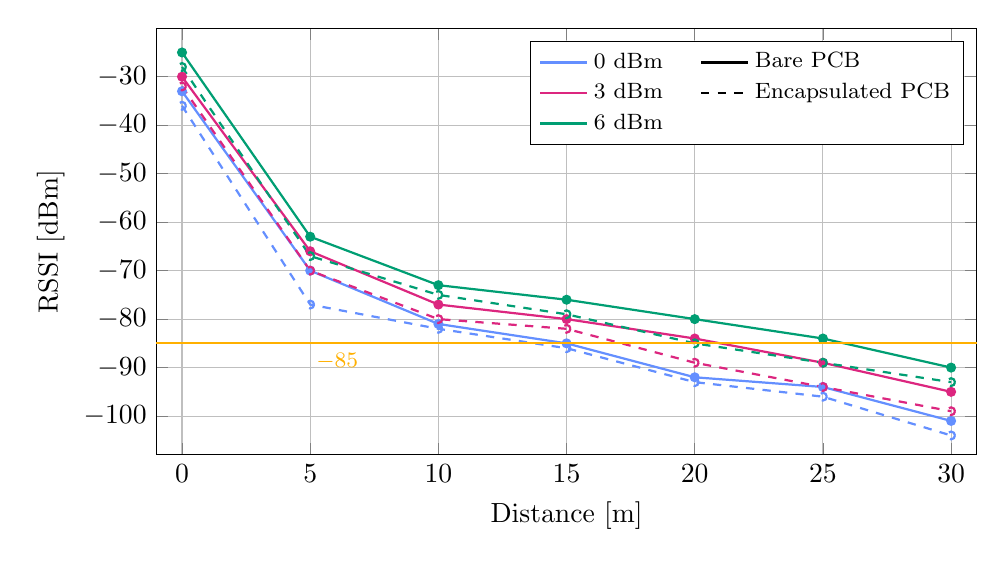
\begin{tikzpicture}

\begin{axis}[
    set layers,
    grid=both,
    xlabel={Distance},
    x unit={\si{\meter}},
    ylabel={RSSI},
    y unit={dBm},
    xmin=-1, xmax=31,
    xtick={0,5,...,30},
    ymin=-108, ymax=-20,
    ytick={-100,-90,...,-30},
    legend cell align={left},
    legend columns=2,
    legend style={
        at={(0.985,0.97)}, anchor=north east,
        font=\footnotesize,
        /tikz/every even column/.append style={column sep=0.4cm},
    },
]

\addplot[IBM1,  thick, mark=*, mark size=1.4pt, forget plot]
    coordinates {(0,-33)(5,-70)(10,-81)(15,-85)(20,-92)(25,-94)(30,-101)};
\addplot[IBM3,  thick, mark=*, mark size=1.4pt, forget plot]
    coordinates {(0,-30)(5,-66)(10,-77)(15,-80)(20,-84)(25,-89)(30,-95)};
\addplot[IBM10, thick, mark=*, mark size=1.4pt, forget plot]
    coordinates {(0,-25)(5,-63)(10,-73)(15,-76)(20,-80)(25,-84)(30,-90)};

\addplot[IBM1,  thick, dashed, mark=o, mark size=1.4pt, forget plot]
    coordinates {(0,-36)(5,-77)(10,-82)(15,-86)(20,-93)(25,-96)(30,-104)};
\addplot[IBM3,  thick, dashed, mark=o, mark size=1.4pt, forget plot]
    coordinates {(0,-32)(5,-70)(10,-80)(15,-82)(20,-89)(25,-94)(30,-99)};
\addplot[IBM10, thick, dashed, mark=o, mark size=1.4pt, forget plot]
    coordinates {(0,-28)(5,-67)(10,-75)(15,-79)(20,-85)(25,-89)(30,-93)};

\addplot[IBM5, thick, on layer=axis foreground, forget plot] coordinates {(-1,-85) (31,-85)}
    node[pos=0, anchor=north west, font=\footnotesize, IBM5, xshift=1.9cm] {\SI{-85}{\dBm}};

\addlegendimage{IBM1, thick}
\addlegendentry{0 dBm}
\addlegendimage{black, thick}
\addlegendentry{Bare PCB}
\addlegendimage{IBM3, thick}
\addlegendentry{3 dBm}
\addlegendimage{black, thick, dashed}
\addlegendentry{Encapsulated PCB}
\addlegendimage{IBM10, thick}
\addlegendentry{6 dBm}

\end{axis}

\end{tikzpicture}
\end{document}
